\chapter{Computational Geometry}
In this chapter, we present some of the Computational Geometry notion about mesh and Delaunay triangulation useful to full understand the reconstruction method described in the thesis. 
\section{2-Manifold Surface}
We give the basis to formulate a formal definition of 2-manifold mesh, since the reconstruction algorithm we propose deals with these type of surfaces. 
\subsection{Topological Space}
A 2-manifold surface is particular specialization of topological space. 
A topological space is usually a set of points together with a  relationship defining a set of neighbors of each points. More formally:
\begin{mydef}
\textbf{Topological Space}

  Given a set $X$ and a set of subsets $\tau$, named open sets; $(X, \tau)$ is a topological space if:
  \begin{itemize}
    \item $\emptyset \in \tau$;
    \item $X \in \tau$;
    \item $\forall t_1,t_2 \in \tau $, $t_1 \cup t_2 \in \tau$;
    \item the intersection of any finite number of subsets in $\tau$.
  \end{itemize}
\end{mydef}
The set $\tau$ is named topology.
For each set $X$ is always possible to define two topologies: the indiscrete or trivial topology, consisting of $X$ and $\emptyset$; the discrete topology, containing all of the possible subsets of $X$.

Other examples of topological spaces are metrical spaces. 
\begin{mydef}
  \textbf{Metrical Space}
  
A metrical space is a pair $(M, d)$, where $M$ is a set of points, and $d$ is a metric on $M$ such that, for any $x$, $y$ and $z \in M$:
\begin{itemize}
  \item $d(x, y) \geq 0$
  \item $d(x, y) = 0 \Longleftrightarrow x = y$
  \item $d(x, y) = d(y, x)$
  \item $d(x, z) \leq d(x, y) + d(y, z)$
\end{itemize}

\end{mydef}


Whenever $M = \mathbb{R}^k$ and $d$ is the Euclidean distance, then, $(\mathbb{R}^k, d)$ is the Euclidean topological space; in the case of 3D reconstruction, $k=3$.
The set of subset $\tau$ defining a topology in this case is composed by all the open balls
\[
B_k(x_0, r) = \{x \\in \mathbb{R}^k | d(x_0, x) < r\}
\]
with $x_0 \in M$ and $r > 0$.
To define a 2-manifold and we need the notion of homeomorphism.

\begin{mydef}
   \textbf{Homeomorphism}
   
   Given two topological spaces $(M_1, d_1)$ and $(M_2, d_2)$, a homeomorphism is a function $f:M_1\longrightarrow M_2$, such that:
   \begin{itemize}
    \item $f$ is bijective;
    \item $f$ is continuous;
    \item $f{-1}$ is continuous.
   \end{itemize}
\end{mydef}

For instance, the open interval $(a, b)$ is homeomorphic to $\mathbb{R}$ for any $a < b$; and $B_k(\mathbf{0}, 1)$ is homeomorphic to $\mathbb{R}^k$. 

\subsection{$k$-manifold}
A $k$-manifold, with $k \in \mathbb{N}$ is a topological space that is locally similar to $\mathbb{R}^k$. More formally:

\begin{mydef}
 \textbf{$k$-manifold in $\mathbb{R}^n$}
 
 Given $M \subseteq \mathbb{R}$ and $1 < k < n, k \in \mathbb{R}$, them, $(M, \tau_M)$ is a $k$-manifold if $\forall \mathbf{x} \in M$, then $\mathbf{x} \in V$ and $V$ is homeomorphic to $B_k(\mathbf{0}, 1)$.
\end{mydef}

In the thesis we deal with 2-manifolds in $\mathbb{R}^3$, named surfaces, in particular with connected surfaces. 

\begin{mydef}
\textbf{Connected Space}

A topological space is connected if it cannot be represented as the union of two disjoint nonempty open sets. 
\end{mydef}

Every 2-manifold can be categorized according to its genus. Intuitively, the genus is the number of holes in the surface. Formally


 
\begin{mydef}
\textbf{Genus}

Given a connected surface $M$, its genus is an integer number $h$ equals to the maximum number of cuts along non intersecting curves such that the resulting surfaces keeps the connected property.
\end{mydef}

\begin{figure}
 \begin{tabular}{cccc}
  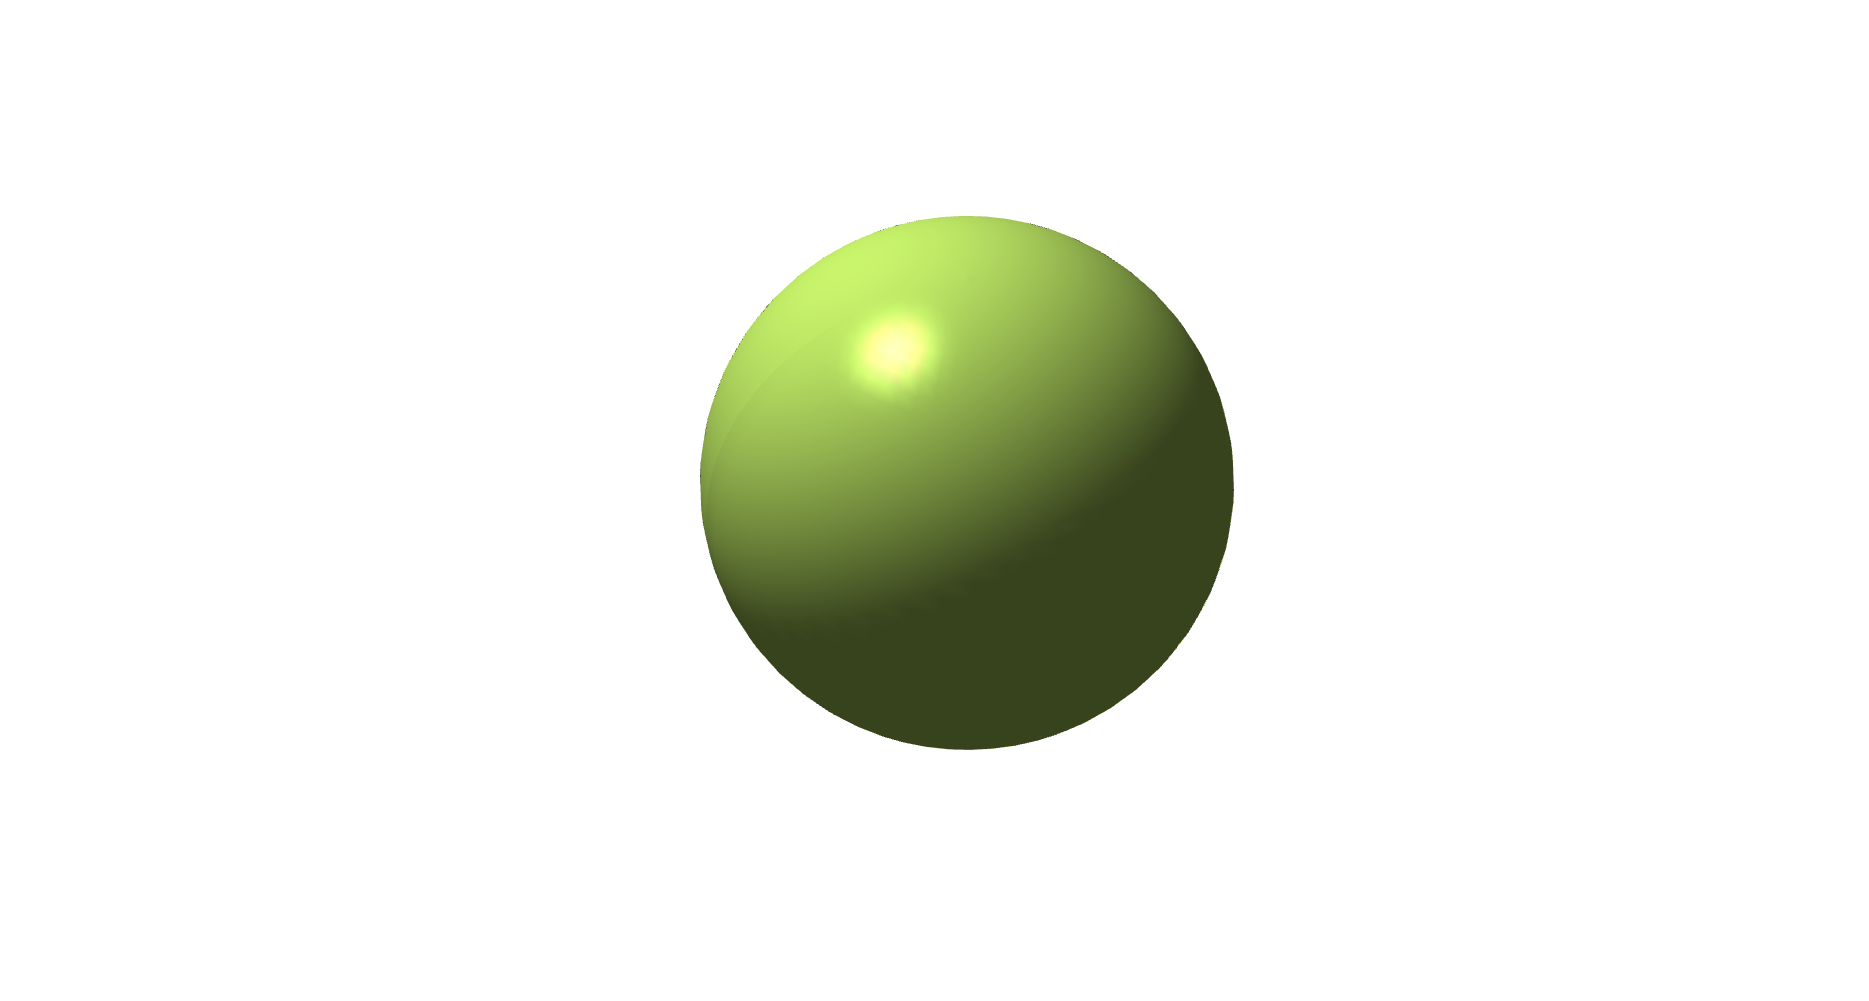
\includegraphics[width=0.22\columnwidth]{./img/sphere}&
  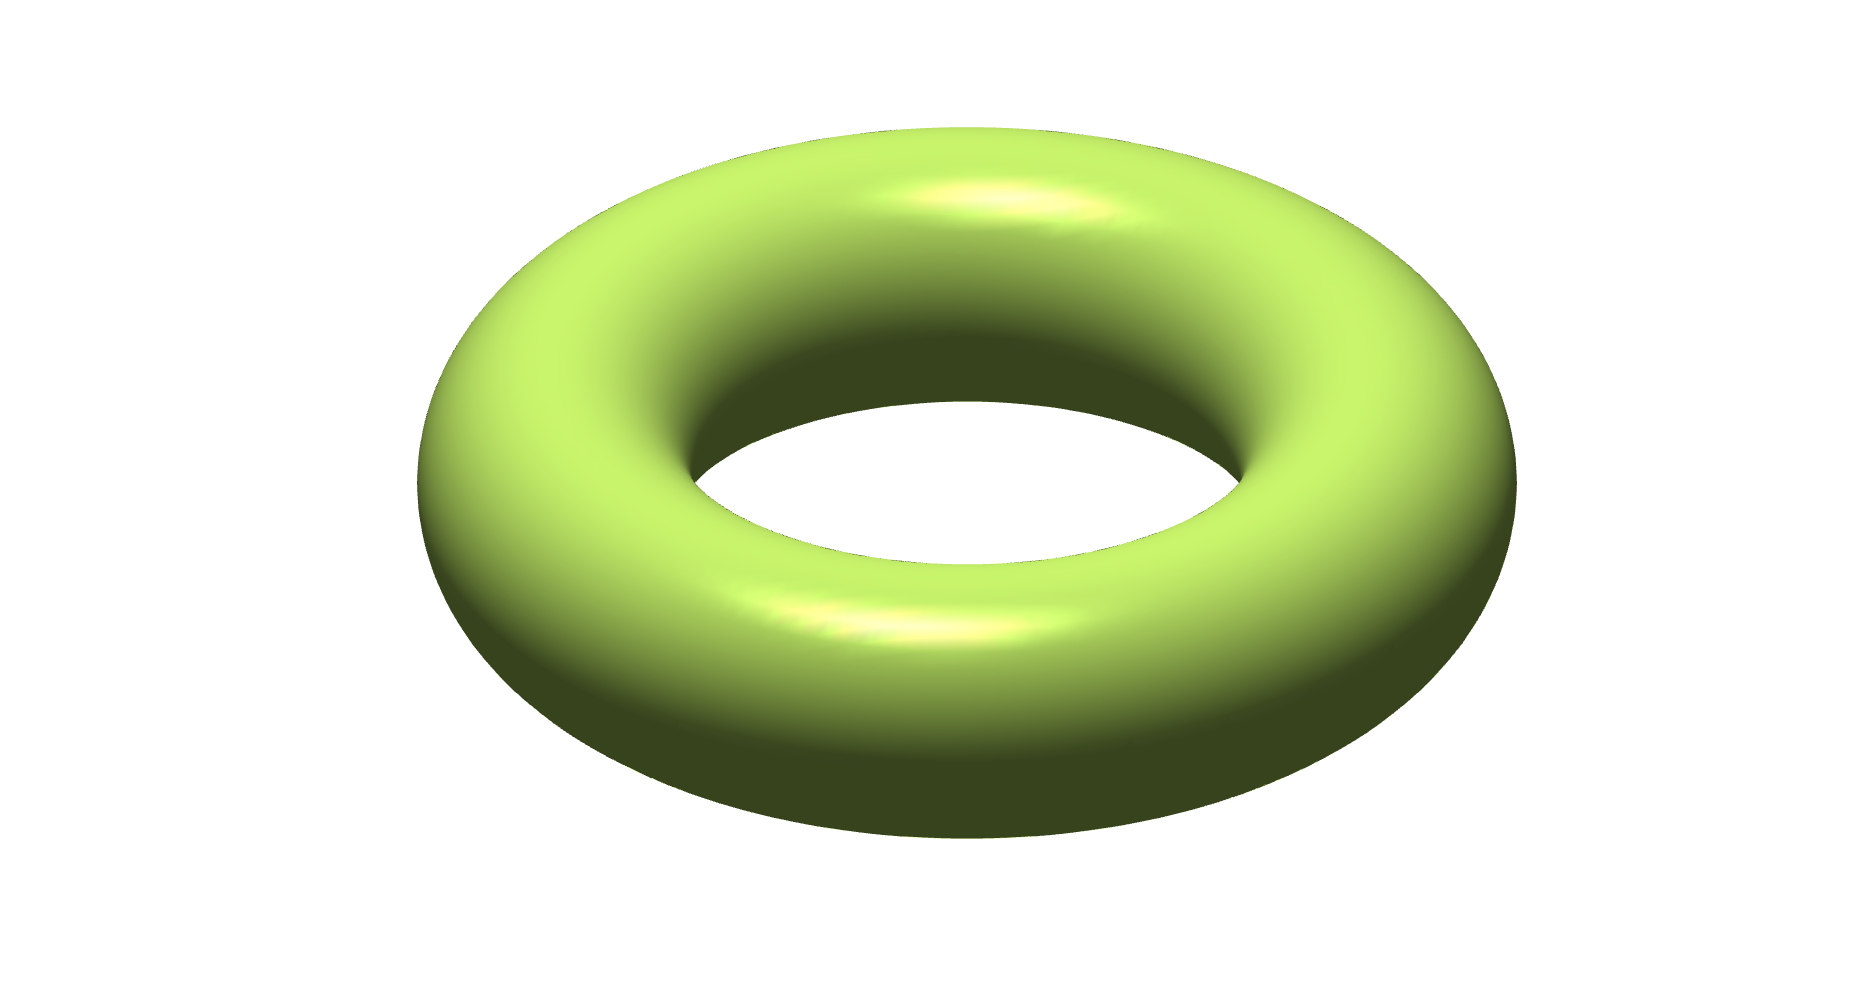
\includegraphics[width=0.22\columnwidth]{./img/torus}&
  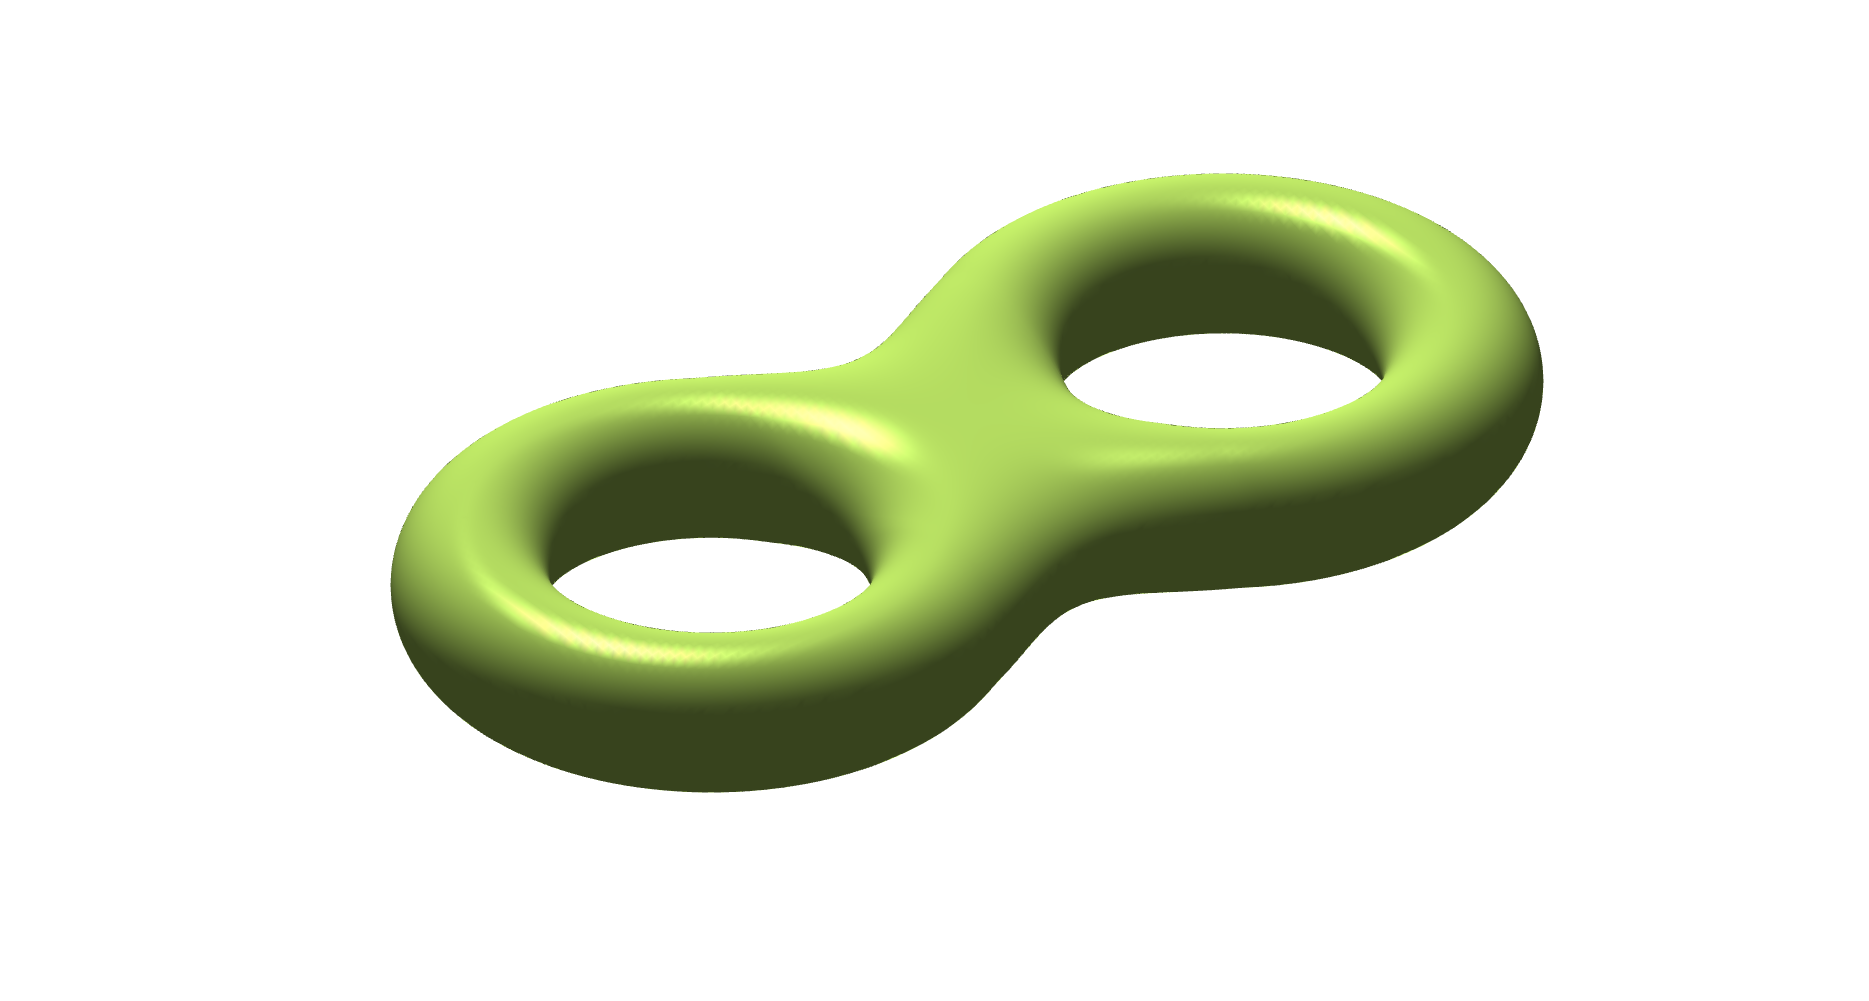
\includegraphics[width=0.22\columnwidth]{./img/doubleTorus}&
  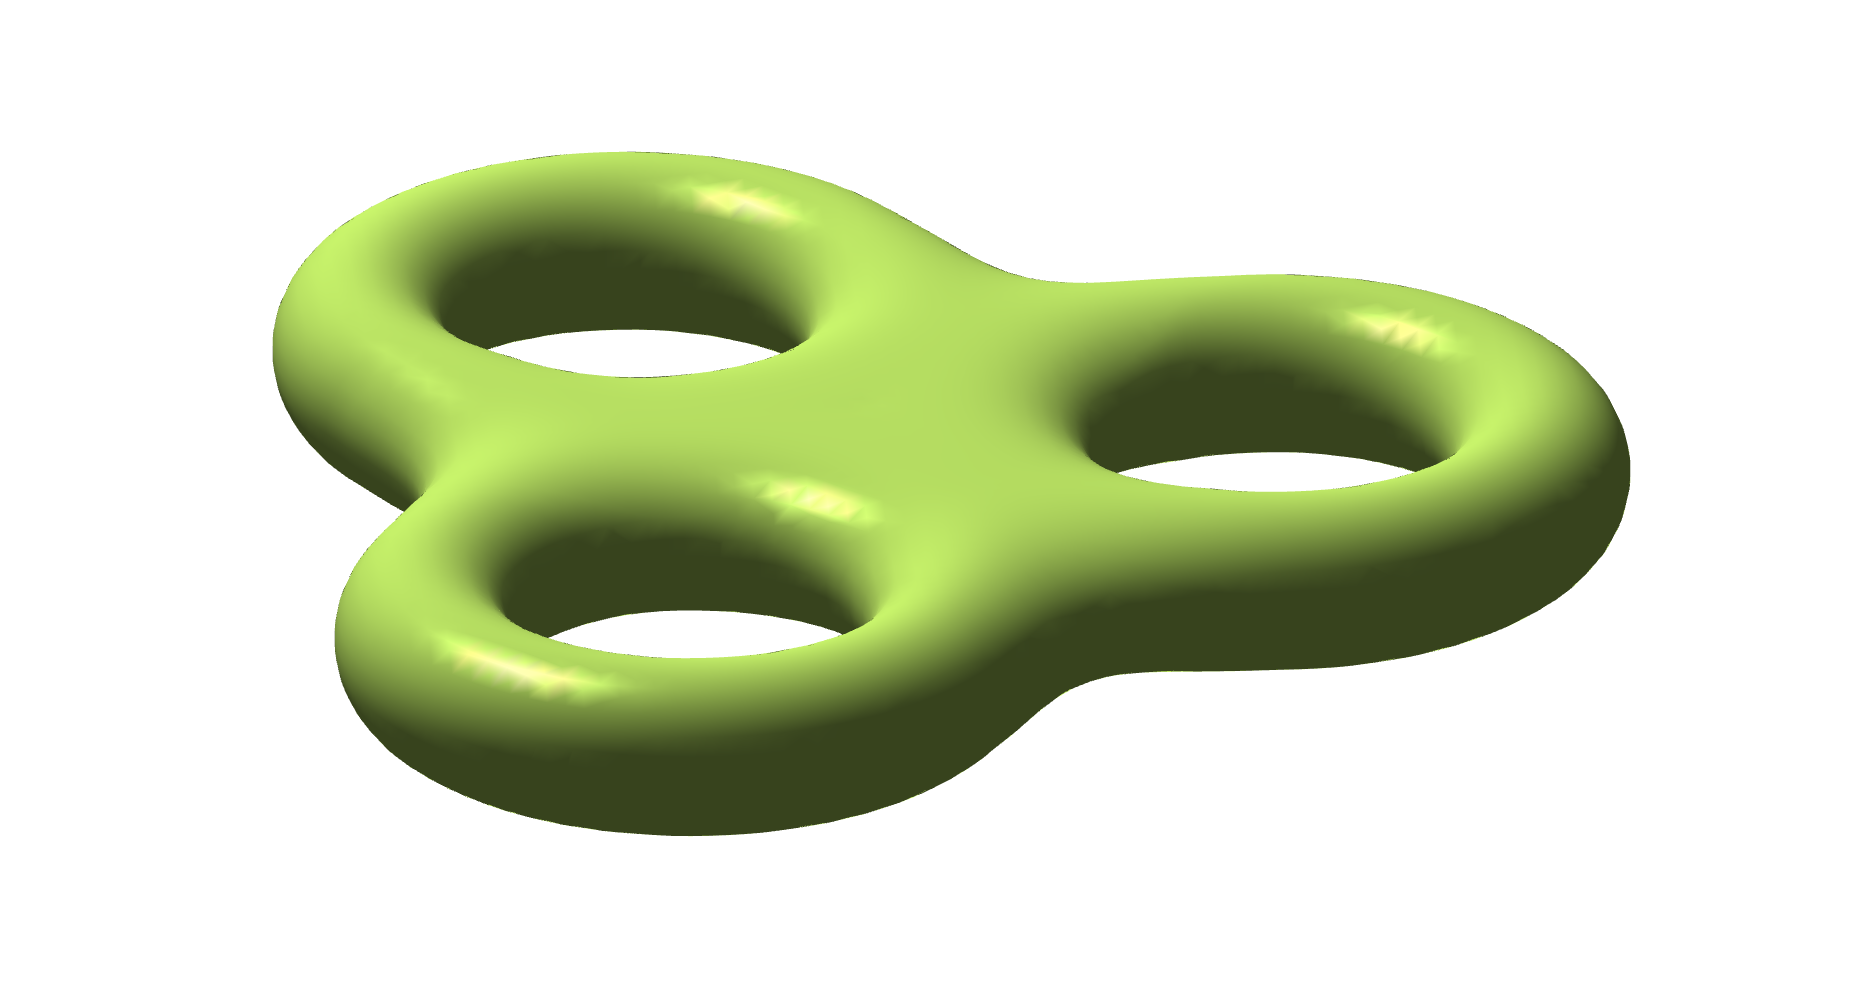
\includegraphics[width=0.22\columnwidth]{./img/tripletorus}\\
  Genus 0 & Genus 1 & Genus 2 & Genus 3
 \end{tabular}
 
\end{figure}



% \begin{thm}
% Here is a new definition
% \end{thm}

\subsection{Manifold in the Discrete Domain}
The surface described thus far, can be discretized through a simplicial complex which is a particular set of simplex.

Given $k + 1$ distinct points $v_0, \dots, v_k \in \mathbb{R}^n$, they are \emph{affinely independent} if a set of real numbers $\{c_0, \dots, c_k \}$ exists, such that the following equations:
\[
\sum_{i=0}^k{c_i v_i} = 0 \text{and} \sum_{i=0}^k{c_i} = 0
\]
are valid if and only if   $c_0 = \dots = c_k = 0$.


\begin{mydef}
 \textbf{$k$-simplex} 
 
 Let $\{v_0, \dots, v_k\}$ be a set of affinely independent points. The simplex spanned by this set of points is their convex hull
 \[
 \sigma = [v_0, \dots, v_k] = \left\{ \sum_{i=0}^{k}{t_i v_i} : t_i \geq 0 \text{and}  \sum_{i=0}^{k}{t_i} = 1\right\}.
 \]
\end{mydef}
In the previous relation, the values $t_i$ represent the barycentric coordinates and the each point in $\{v_0, \dots, v_k\}$ is named vertex.

Each simplex spanned by a nonempty subset of the vertices in $\sigma$ is called face, if $l\leq k$ is the cardinality of this subset, then is called $l$-face

The simplices in $\mathbb{R}^3$ are:
\begin{itemize}
  \item point: 0-simplex, with one 0-face;
  \item segment: 1-simplex, with two 0-faces and one 1-face;
  \item triangle: 2-simplex, with three 0-faces, three 1-faces and one 2-face
  \item tetrahedron: 3-simplex, with four 0-faces, six 1-facex, four 2-faces and one 3-face
\end{itemize}
\todo{figure}

\begin{mydef}
\textbf{Simplicial complex}

A simplicial complex $C$ is a finite set of simplices satisfying two properties:
\begin{itemize}
  \item any face $\phi < \sigma$ of a simplex $\sigma \in C$ is also a simplex in $C$, i.e. $\phi \in C$
  \item if two simplices $\phi, \sigma \in C$, their intersection $\phi \cap \sigma$ is a face of both $\phi$ and $\sigma$
\end{itemize}
\end{mydef}
Some examples of simplicial complexes are the triangulations of a set of points in 2D, or the tetrahedrization in 3D.

If $C$ is a simplicial complex, the notation $\delta C$ represents the union of the simplices in $C$, and is named polyhedron. The polyhedron $\delta C$ is a topological space \todo{which topology pag 8 yu}, and 

\begin{mydef}
\textbf{Triangulated $k$-manifold}

A triangulated $k$-manifold is a simplicial complex $C$ such that $\delta C$ is $k$-manifold.
\end{mydef}

From now, $k$-manifold stands fo the triangulated $k$-manifold.

\subsubsection{Manifold test}
Given a simplicial complex $C$, and its relative polyhedron, we are able to check if $\delta C$ is $k$-manifold through the tests described in \cite{lhuillier20152}.
First, we define the notion of good edges, and good vertex.


\begin{mydef}
\textbf{Good Edges}
An edge in $\delta C$ is a good edge if it is included in exactly two triangles of $\delta C$
\end{mydef}

\begin{mydef}
\textbf{Good Vertex}
A vertex in $\delta C$  is a good vertex if the incident triangles in $\delta C$  can be ordered as
$t_0 , t_1, \dots, t_k$ such that $t_i \cap t_{(i+1) mod (k+1)}$ is an edge $\forall i \in {0, 1, \dots, k}$.
\end{mydef}




% 
% According to [Vegter,handbook],
% Theorem 1 (Global Test) |∂ O| is a 2-manifold iff the ver-
% tices and the edges in c(∂ O) are ∂ O-good.
% We have the same test for a single vertex:
% Theorem 2 (Triangle-based Test) A vertex v in c(∂ O) is
% regular in |∂ O| iff v and the v-incident edges in c(∂ O) are
% ∂ O-good.












\section{Delaunay Triangulation}
\subsection{Point modifications}
\section{Mesh processing}
\subsection{Smoothing}
\subsection{Remeshing}
\subsection{Merging}